\documentclass[a4paper]{article}
\usepackage[utf8]{inputenc}
\usepackage[russian,english]{babel}
\usepackage[T2A]{fontenc}
\usepackage[left=10mm, top=20mm, right=10mm, bottom=15mm, footskip=13mm]{geometry}
\usepackage{indentfirst}
\usepackage{amsmath,amssymb}
\usepackage{graphicx}
\usepackage[italicdiff]{physics}
\graphicspath{ {shema/} }
\graphicspath{ {graphic/} }
\usepackage{caption}
\captionsetup[figure]{name=Рисунок}
  
\title{\underline{Отчет о выполненой лабораторной работе 1.1.1}}
\author{Антон Хмельницкий, Б01-306}

\begin{document}
\maketitle
\textbf{Измерение удельного сопротивления нихромовой проволоки}

\section{Аннотация}

В данной лабораторной работе измеряется удельное сопротивление нихромовой проволки. 
Для этого используются методы:
\begin{enumerate}
\item Определение углового коэффициента наклонной в зависимости U(I) - напряжения от тока, измеряемых с помощью цифрового амперметра и аналогового вольтметра.
\item Измерение сопротивления с помощью моста постоянного тока.
\end{enumerate}\par
С помощью линейки, штангенциркуля и микрометра измеряются геометрические размеры проволоки.
Отдельное внимание уделяется случайным и систематическим погрешностям в измерениях.\par

\section{Теоретические сведения}

Удельное сопротивление материала проволоки круглого сечения изготовленной из однородного материала и имеющей постоянную толщину определяется по формуле:
\[ \rho = \frac{R_\text{пр}}{l}\frac{\pi d^2}{4}  \]
где $R_\text{пр}$ -сопротивление измеряемого отрезка проволоки, $l$ - его длина, $d$ - диаметр.
Поэтому измеряем длину, диаметр и электрическое сопротивление проволоки.\par
Диаметр у проволоки не постоянный поэтому нужно учесть случайную погрешность.
\begin{figure}[t]
    \centering
    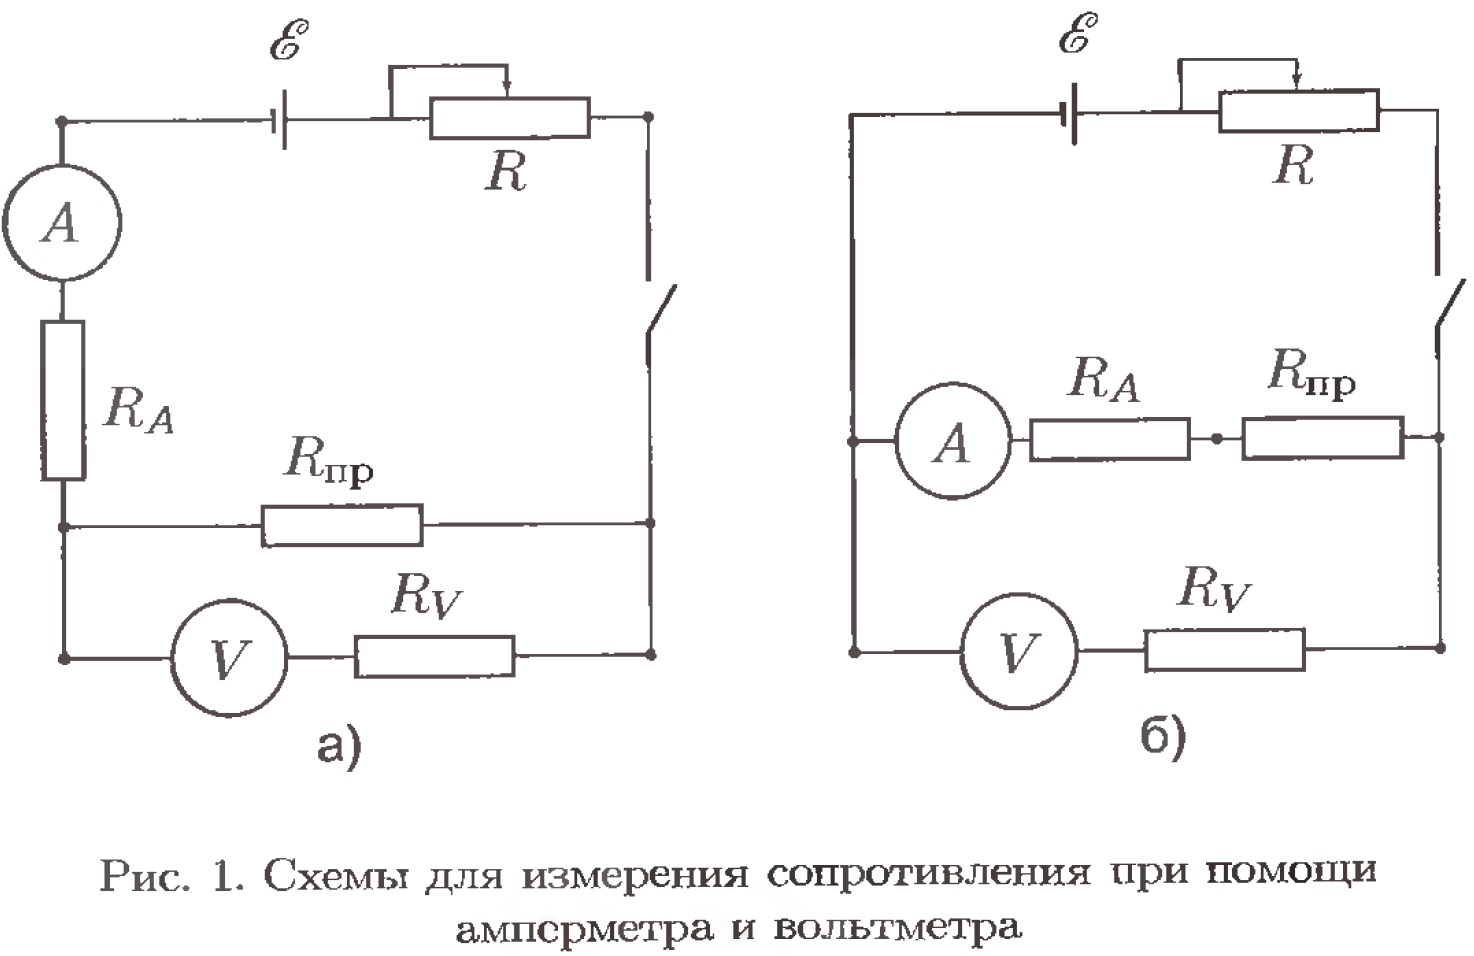
\includegraphics[width=0.5\textwidth]{shema}
    \caption{Схема для измерения сопротивления}
\end{figure}

По закону Ома: $R_\text{пр} = \frac{V_{a}}{I_{a}}$, где $V_{a}$ и $I_{a}$ - показания вольтметра и амперметра. Для измерения используем схему а) из учебника "Лабораторный практикум по общей физике т.1 Гладов" - рис.1, т.к. погрешность в измерениях там меньше чем в схеме б) (расчет будет в соответствующем параграфе).Получаем формулы для расчета: $R_\text{пр1} = \frac{V_{a}}{I_{a}} = R_\text{пр}\frac{R_{v}}{R_\text{пр} + R_{v}}$. Преобразовываем: $ R_\text{пр} = \frac{R_\text{пр1}}{1-(R_\text{пр1}/R_{v})} \approx R_\text{пр1}(1 + \frac{R_\text{пр1}}{R_{v}})$ (Используется приближение, т.к. сопротивление вольтметра $R_{v} \gg R_\text{пр},R_\text{пр1}$).\newline
График зависимости $V_{a}(I_{a})$ должен представлять прямую, угловой коэффициент которой и будет равен $R_{пр1}$.

\section{Оборудование и системные погрешности}

\begin{itemize}
  \item Линейка:  $\sigma_\text{лин} = \pm 0.5$ мм (по цене деления).
  \item Штангенциркуль: $\sigma_\text{штан} = \pm0.1$ мм (маркировка производителя).
  \item Микрометр:  $\sigma_\text{микр} = \pm0.01$ мм (маркировка производителя).
\end{itemize}  
\begin{center}
    \begin{tabular}{|c | c | c |}
     \hline
      & Вольтметр & Амперметр \\
    \hline
     Система & Магнитоэлектрическая & Электромагнитная \\ 
     \hline
     Класс точности & 0.5 & 0.5 \\
     \hline
    Погрешность измерений & 0.2\%(по маркировке) &$\sigma_{A} = \pm(0.002x+0.02)$, x - величина измерения.\\
     \hline
     Число делений шкалы n & 150 на 600 мВ & цифровой дисплей, 5 ед. на 000.00 мА \\
     \hline
     Внутреннее сопротивление прибора & 4 кОм & 1.2 Ом \\
     \hline
    \end{tabular} 
\end{center}
Сравним погрешности для а) и б):\par
    для а): $R_\text{пр}/R_{V} = 10/4000 = 0.0025 ,  \text{т.е. } 0.25\%$.\par
    для б): $R_{A}/R_\text{пр} = 1.2/10 = 0.12,$ т.е. $12\%$.\par
    Значит схема а) более точна с погрешностью 0.25\% \par
    Так как погрешность от половины цены деления больше чем погрешность измерений, то итоговая погрешность вольтметра будет $\sigma_{V} = \pm(600/150)/2 $мВ$= \pm 2$ мВ.\par
    Для значений амперметра от 50 мА до 300 мА погрешность будет составлять от $\sigma_{A} = \pm 0.06 \text{мА}$ до  $\sigma_{A} = \pm 0.6 \text{мА}$.
Мост постоянного тока P4833: Класс точности - 0.1, Разрядность магазина сопротивлений - 5 ед., Множитель - $N = 10^{-2}$, Погрешность $\sigma_\text{м} = 0.1\% \Rightarrow  \sigma_\text{м} = 0.001$ Ом.


\section{Результаты измерений и обработка данных}
\subsection{Измерение диаметра проволоки}
\begin{center}
    \begin{tabular}{|c | c | c | c | c | c | c | c | c | c | c |} 
     \hline
      & 1 & 2 & 3& 4& 5& 6 & 7 & 8 & 9 & 10 \\
    \hline
     $d_\text{штанг}$, мм & 0.4 & 0.4 & 0.4 & 0.4 & 0.4 & 0.4 & 0.4 & 0.4 & 0.4 & 0.4  \\ 
     \hline
     $d_\text{микр}$, мм & 0.35 & 0.34 & 0.35 & 0.34 & 0.34 & 0.33 & 0.34 & 0.35 & 0.34 & 0.34 \\
     \hline
    \end{tabular} 
\end{center}
Погрешности: 
Для штангенциркуля в 10 замерах был результат 0.4, погрешности будут считаться для микрометра как более точного инструмента.
\begin{itemize}
\item Среднее значение: $\langle d \rangle = \frac{1}{n}\sum\limits_{i=1}^n d_{i} = 0.342$ мм. 
\item Стандартное отклонение: $\sigma_\text{d} = \sqrt{\frac{1}{n}\sum\limits_{i=1}^n(d_{i} - \langle d \rangle)^2} = 0.0063$ мм.
\item Стандартная погрешность опыта: $\sigma_\text{ср} = \frac{\sigma_\text{d}}{\sqrt{n}} =  0.002$ мм.
\item Полная погрешность: $\sigma_\text{полн} = \sqrt{\sigma_\text{ср}^2 + \sigma_\text{микр}^2} = 0.0102$ мм.
\end{itemize}
Итоговые результаты: \par
Штангенциркуль: $d_{\text{штанг}} = 0.4 \pm 0.5$ мм.\par
Микрометр: $d_{\text{микр}} = 0.342 \pm 0.0102$ мм. $(\varepsilon_{d} = 3\% )$

\subsection{Измерение сопротивления проволоки}

\begin{center}
    \begin{tabular}{|c |c | c | c | c | c | c | c | c | c | c | c |} 
     \hline
      & \multicolumn{11}{c|}{l = 20 см}\\
     \hline
     $V_{\text{В1}}$, мВ & 0 & 340 & 240 & 280 & 560 & 520 & 480 & 440 & 320 & 400 & 360  \\ 
     \hline
     $I_{\text{А1}}$, мА & 0 & 157.8 & 111.13 & 129 & 260 & 241 & 223.45 & 204.56 & 148.4 & 185.5 & 166.45 \\
     \hline
     & \multicolumn{11}{c|}{l = 30 см}\\
     \hline
     $V_{\text{В2}}$, мВ & 0 & 560 & 340 & 240 & 280 & 320 & 360 & 400 & 440 & 520 & 480  \\ 
     \hline
     $I_{\text{А2}}$, мА & 0 & 173.4 & 104.5 & 74 & 86.35 & 98.73 & 111 & 123.2 & 135.38 & 161.35 & 148.3 \\
     \hline
     & \multicolumn{11}{c|}{l = 50 см}\\
     \hline
     $V_{\text{В3}}$, мВ & 0 & 320 & 360 & 400 & 440 & 480 & 520 & 560 & 340 & 380 & 420  \\ 
     \hline
     $I_{\text{А3}}$, мА & 0 & 59.35 & 67 & 74.3 & 81.7 & 89.1 & 97.05 & 104.36 & 63.24 & 70.5 & 78.09 \\
     \hline 
    \end{tabular} 
\end{center}

Результаты исследований зависимостей показаний вольтметра $V_{a}$  от показаний амперметра $I_{a}$ представлены на рисунке 2.
С помощью метода наименьших квадратов были построены аппроксимирующие прямые $V_{B} = \langle R \rangle I_{A}$ по формуле: \[ \langle R \rangle = \frac{\langle VI \rangle}{\langle I^2 \rangle}\]\par
Погрешность угла наклона в аппроксимации(т.е. погрешность $\langle R \rangle$) найдем как косвенную погрешность наименьших квадратов по формуле: $\sigma_{R\text{случ}} = \sqrt{\frac{1}{n-1}(\frac{\langle V^2 \rangle}{\langle I^2 \rangle}-\langle R \rangle^2)}$.\par
Систематическую погрешность найдем как частные производные за значения выбрав наибольшие измерения: \[ \sigma_{R\text{сист}} = R \sqrt{\left(  \frac{\sigma_{V}}{Vmax}\right)^2 + \left(\frac{\sigma_{I}}{Imax}\right)^2}  \] \par
Полную погрешность вычислим по формуле: \[\sigma_{R\text{полн}} = \sqrt{\left( \sigma_{R\text{случ}}\right)^2 + \left( \sigma_{R\text{сист}}\right)^2} \] \par
Занесем итоговые значения и погрешности в таблицу и сравним их с измерениями полученными на мосту P4833:
\begin{center}
    \begin{tabular}{| c | c | c | c | c | c | c |}
     \hline
     l, см & $\langle R \rangle $, Ом & $\sigma_{R\text{случ}}$, Ом & $\sigma_{R\text{сист}}$, Ом & $\sigma_{R\text{полн}}$,Ом & $\varepsilon_{R}$, \% & $R_{\text{мост}}$, Ом \\
     \hline
     20 см & 2.156 & 0.0018 & 0.0092 & 0.0094 & 0.43 & $2.168 \pm 0.001$  \\ 
     \hline 
     30 см & 3.240 & 0.0033 & 0.0161 & 0.0164 & 0.5 &  $3.2538 \pm 0.001$  \\
     \hline
     50 см & 5.377 & 0.0039 & 0.0364 & 0.0366 & 0.68 & $5.3728 \pm 0.001$  \\
     \hline
    \end{tabular} 
\end{center}
Заметим, что случайная составляющая на порядок меньше чем системная, и ,сравнивая измерения с моста, видно, что расхождения со значениями с моста не больше чем $\pm 2\sigma_{R\text{полн}}$.

\begin{figure}[t]
    \centering
    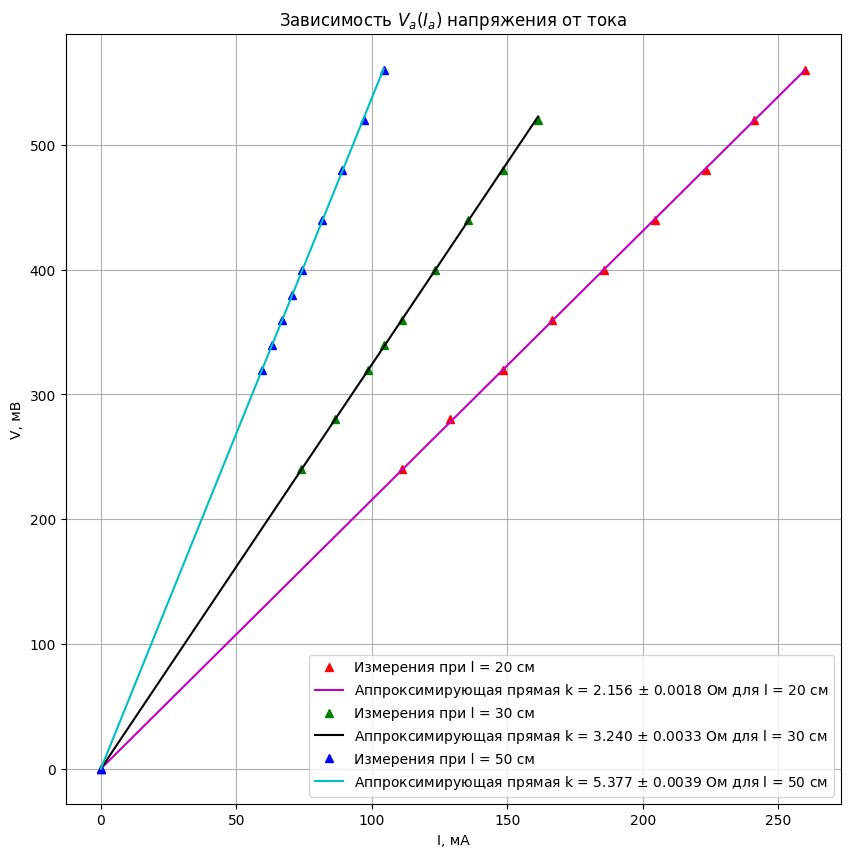
\includegraphics[width=0.9\textwidth]{graphic}
    \caption{График измерений для зависимости $V_{a}(I_{a})$ для проволок разной длины с аппроксимацией y = kx. Погрешности измерений равняются инструментальным погрешностям: $\sigma_{V} = \pm 2$ мВ и $\sigma_{A} = \pm 0.6$ мА. Т.к. эти величины на 2 порядка меньше измеряемых, то они не будут указаны на графике из-за потери наглядности и информативности.}
\end{figure}

\subsection{Вычисление удельного сопротивления}
Найдем удельное сопротивление нихромовой проволоки по формуле из теор.части, используя $d_{\text{микр}} \text{и} \langle R \rangle$.\par 
Заметим что относительная погрешность сопротивления $\varepsilon_{R} < 1\%$ и по сравнению с относительной погрешностью диаметра проволоки  $\varepsilon_{d} = 3\%$ мало, значит можно ей пренебречь. Поэтому учитывать будем только $\sigma_{R\text{полн}}$. \par

Используя формулу погрешности косвенных величин: \[ \sigma_{a}^2 = \left( \pdv{f}{b} \right)^2\sigma_{b}^2 + \ldots \]
Для зависимости удельного сопротивления получаем: \[ \sigma_{\rho}^2 = \left( \pdv{\rho}{d} \right)^2\sigma_{d}^2 = \left( \frac{R\pi 2d}{4l} \right)^2\sigma_{d}^2 \]
Итого получаем $\sigma_{\rho} \approx \frac{2\sigma_{d}}{d}\rho $. Теперь занесем данные в таблицу и затем усредним результаты: 

\begin{center}
\begin{tabular}{|c|c|}
\hline
l, см & $\rho, 10^{-6}$ Ом$\cdot$м \\ \hline
20    & 0.9898 $\pm$ 0.0590  \\ \hline
30    & 0.9916 $\pm$ 0.0592  \\ \hline
50    & 0.9879 $\pm$ 0.0589  \\ \hline
\end{tabular}
\end{center}

Берем среднее за 3 эксперимента \underline{$\langle \rho \rangle = (0.99 \pm 0.059) \cdot 10^{-6}$ Ом $\cdot$ м. $(\varepsilon_{\rho} = 5.9\%)$}

\subsection{Выводы}
В процессе работы было рассчитано удельное сопротивление нихромовой проволоки с точностью $\sim6\%$. Табличное значение  удельного сопротивления нихромового сплава $\rho_{\text{табл}}$ лежит в пределах от 0.97 до $1.14 \cdot 10^{-6} \text{Ом} \cdot \text{м}$. Значит, полученный результат $ \rho_{\text{итог}} = (0.99 \pm 0.059) \cdot 10^{-6}$ Ом $\cdot$ м. попадает в табличный диапазон.\par
В данной работе было уделено особое внимание погрешностям. Сравнивая их видно, что случайная погрешность обычно на порядок меньше чем, поэтому приходим к выводу, что основная часть погрешности возникает из-за неидеальности приборов, в данном случае погрешность микрометра в 6 раз больше погрешности вольтметра и амперметра и системная погрешность микрометра больше случайной в 5 раз. Поэтому учитывалась только погрешность микрометра и именно она как видно в итоге оказала наибольшее влияние на погрешность удельного сопротивления.

\end{document}


